\chapter{Экспериментальная проверка применимости метода на суперкомпьютере}
	Применимость метода оценивалась с помощью запусков приложений на суперкомпьютере “Ломоносов-2”. Вычислительные узлы суперкомпьютера включают процессор Intel Haswell-EP E5-2697v3 (2.6 GHz), обородуваны 64 GB памяти и связаны коммуникационной сетью InfiniBand FDR \cite{Lom2_stat}.

	В качестве приложений для тестирования использовались реализации HPL, HPCG, алгоритмов DNS и SUMMA матричного умножения, Graph500. Так как рассматривается слабая масштабируемость, то тестирования проводились с конфигурациями запуса, удовлетворяющими выражению \ref{weak_sc}. Для того чтобы более полно проверить применимость метода на реальнах суперкомпьютерных приложениях и оценить их возможности к слабой масштабируемости, для некоторых из приложений тестирования проводились для нескольких значений констант используемых в выражении \ref{weak_sc} (HPL - 3 различных константы; HPCG, Graph500, DNS - 2 различных константы; SUMMA - 1 константа).



	\section{HPL}

	HPL (High Performance Computing Linpack Benchmark) — тест производительности вычислительной системы, на основе результатов которого формируется современный список TOP500 \cite{top500} лучших в суперкомпьютеров мире. Суть теста заключается в решении плотных систем линейных алгебраических уравнений, используя LU факторизацию, на системах с распределённой памятью.

	HPL имеет сложность алгоритма \(O(N^3)\), а количество операций чтения/записи пропорционально \(O(N^2)\). То есть, если размер задачи увеличить в два раза, то количество операций с плавающей точкой увеличится в восемь раз, в то время, как количество операций с памятью увеличится только в четыре раза. Подобные значения ассимптотик свойственны приложениям с большим количеством вычислений над плотными структурами данных.

	\begin{table}
		\begin{tabular}{|r|c|c|c|c|c|c|}
		\hline
		& \multicolumn{2}{c|}{\(C_1\)} & \multicolumn{2}{c|}{\(C_2\)} & \multicolumn{2}{c|}{\(C_3\)} \\ \hline
		\textnumero & PN & PS & PN & PS & PN & PS \\ \hline
		1 & 6 & 18 & 4 & 20 & 4 & 25 \\ \hline
		2 & 8 & 20 & 6 & 23 & 9 & 33 \\ \hline
		3 & 12 & 23 & 8 & 25,3 & 12 & 36,4 \\ \hline
		4 & 16 & 25 & 10 & 27,35 & 16 & 40 \\ \hline
		5 & 20 & 27 & 12 & 28,9 & 25 & 46,4 \\ \hline
		6 & 27 & 30 & 15 & 31,1 & 35 & 52 \\ \hline
		7 & 40 & 34 & 20 & 34,35 & 42 & 55,2 \\ \hline
		8 & 42 & 35 & 25 & 36,82 & 49 & 58,1 \\ \hline
		9 & 50 & 37 & 30 & 39,1 & 56 & 60,7 \\ \hline
		10 & 60 & 39 & 36 & 41,6 & 64 & 63,5 \\ \hline
		11 & 64 & 40 & 49 & 46,1 & 81 & 68,7 \\ \hline
		12 & 80 & 43 & 64 & 50,4 & 110 & 76,1 \\ \hline
		13 & 90 & 45 & 70 & 51,95 & 121 & 78,5 \\ \hline
		14 & 98 & 46 & 80 & 54,3 & 144 & 83,2 \\ \hline
		15 & 110 & 48 & 81 & 54,5 & 169 & 87,8 \\ \hline
		16 & 125 & 50 & 121 & 62,3 & 182 & 90 \\ \hline
		17 & 140 & 52 & 144 & 66,05 & 196 & 92,2 \\ \hline
		18 & 156 & 53,85 & 169 & 69,6 & 210 & 94,4 \\ \hline
		\end{tabular}
		\caption{Тестовые конфигурации запуска HPL, для трёх различных значений констант}
		\label{test_HPL}
	\end{table}

	\begin{table}
		\begin{tabular}{|r|c|c|c|c|c|c|c|c|c|c|c|c|}
		\hline
		& \multicolumn{4}{|c|}{\(C_1\)} & \multicolumn{4}{|c|}{\(C_2\)} & \multicolumn{4}{|c|}{\(C_3\)} \\ \hline
		\textnumero & PN & PS & RE-time & RE-perf & PN & PS & RE-time & RE-perf & PN & PS & RE-time & RE-perf \\ \hline
		1 & 225 & 60,8 & 7,58 &	6,82 & 225 & 76,65 & 3,82 & 0,82 & 225 & 100,8 & 5,79 & 5,69 \\ \hline
		2 & 400 & 73,7 & 1,79 & 1,90 & 400 & 92,85 & 7,53 & 16,35 & 400 & 117 & 7,73 & 7,73 \\ \hline
		3 & 576 & 83,2 & 0,37 & 0,45 & 576 & 104,8 & 0,62 & 9,25 & 576 & 132 & 6,06 & 5,72 \\ \hline
		4 & 784 & 92,2 & 0,12 & 0,09 & 784 & 116,1 & 1,42 & 10,59 & 784 & 146,3 & 7,42 & 6,95 \\ \hline
		5 & 1369 & 111 & 0,16 & 0,07 & 1369 & 140 & 11,35 & 4,41 & 1369 & 176,2 & 0,02 & 1,69 \\ \hline
		\end{tabular}
		\caption{Целевые конфигурации запуска HPL для трёх различных значений констант и значения относительных ошибок предсказания времени и производительности на этих конфигурациях}
		\label{target_HPL}
	\end{table}

	\begin{figure}[t]
		\centering
		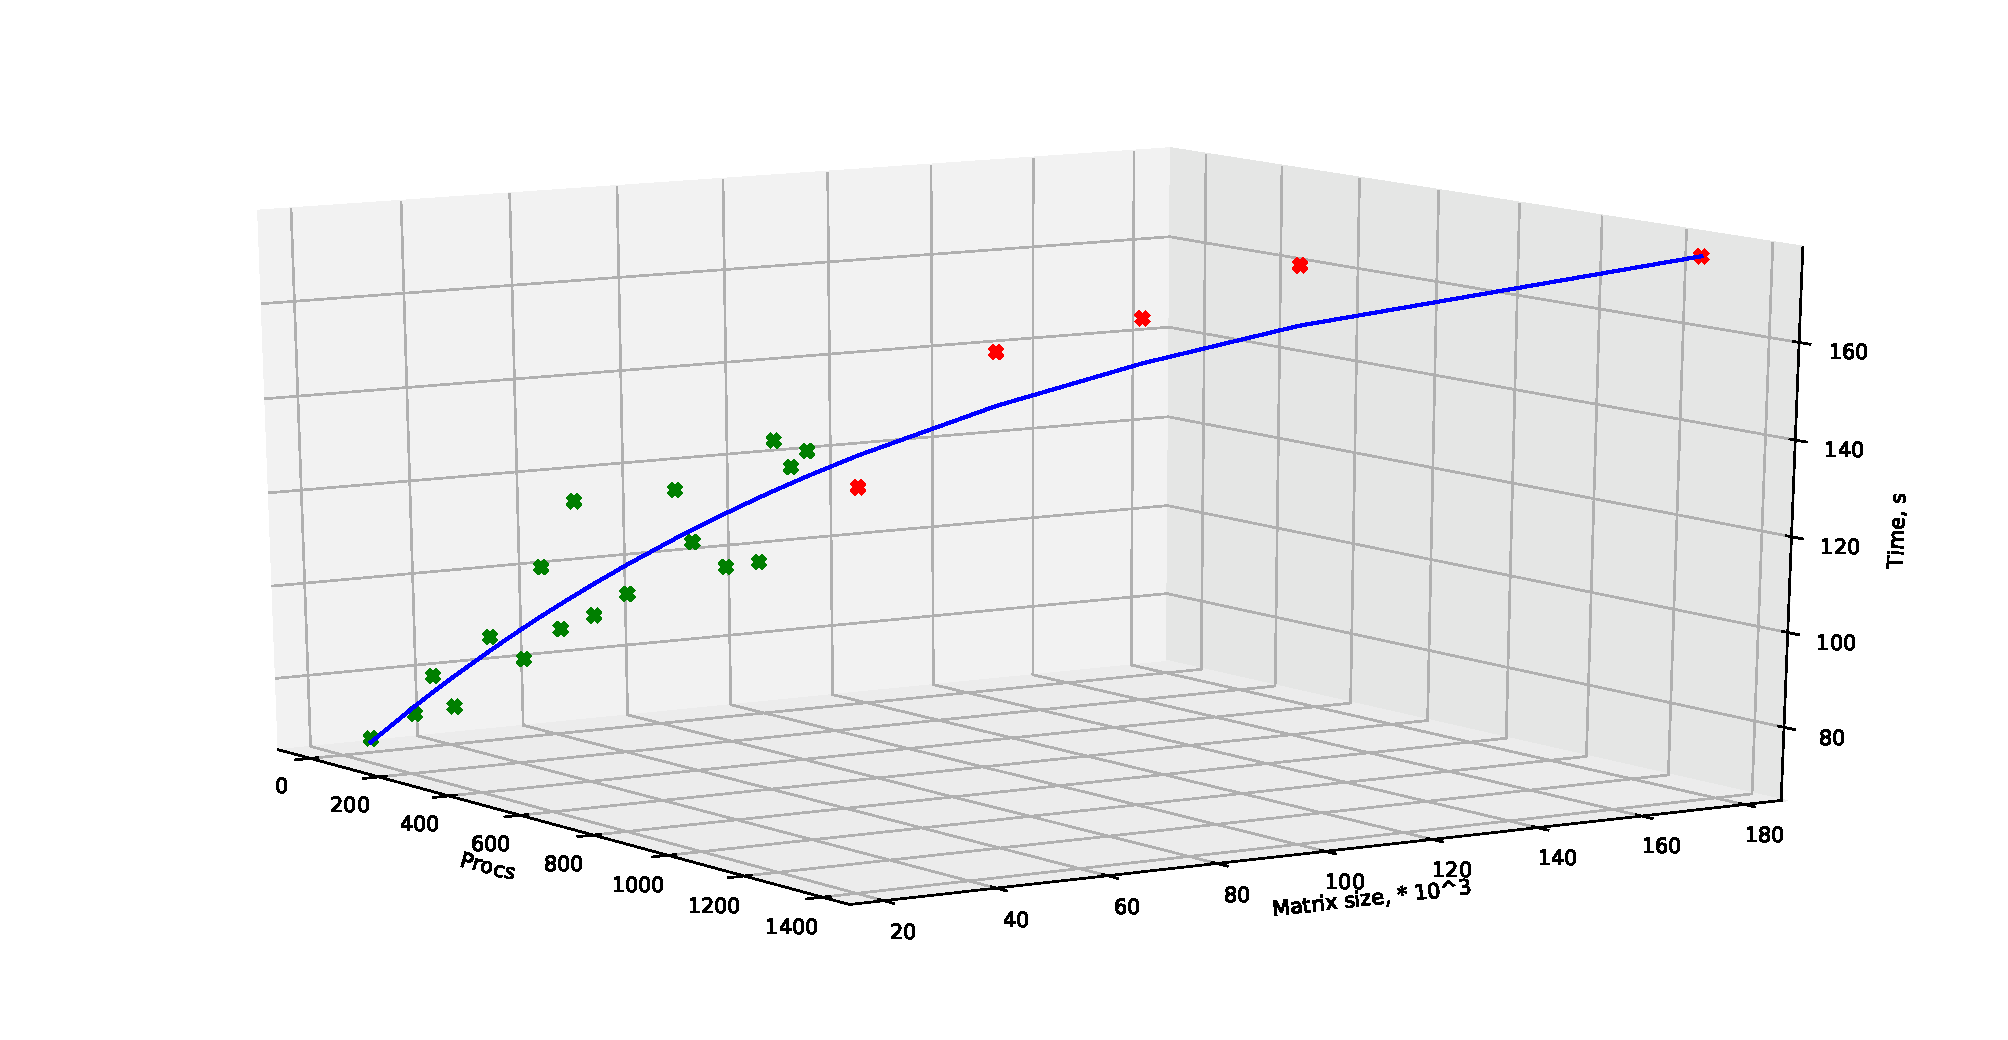
\includegraphics[width=0.9\textwidth]{hpl_k3}
		\caption{Аппроксимирующая функция для слабой масштабируемости HPL, конфигурации соответствуют константе \(C_3\)}
		\label{HPL_C_3_figure}
	\end{figure}

	Тестовые конфигурации запуска, используемые для вычислений параметров модели, и целевых конфигураций, необходимые для оценки погрешности предсказаний, приведены в таблицах \ref{test_HPL} и \ref{target_HPL} соответственно. Коэффициенты \(C_1, C_2, C_3\), связывающие количество работы приходящееся на один процесс и количество используемых процессов, из выражения \ref{weak_sc}, связаны отношением: \(4 \cdot C_1 = 2 \cdot C_2 = C_3 \), то есть с увеличением на единицу номера коэффициента количество работы на один процесс увеличивается в два раза.

	Относительные ошибки для всех целевых конфигураций слабой масштабируемости HPL представлены в таблице \ref{target_HPL}. Значения относительных ошибок предсказания времени по всем целевым конфигурациям варьируются от 0,02\% до 11,35\%, среднее значение - 4,12\%, медиана - 3,82\%, а производительности - от 0,07\% до 16,35\%, среднее значени - 5,23\%, медиана - 5,69\%. Если рассматривать более детально, как меняеются относительные ошибки с увеличением числа используемых процессов и размера задачи, усредняя значение ошибок по конфигурациям с одинаковым количеством использемых процессов, 225 - 5,09\%, 400 - 7,17\%, 576 - 3,74\%, 784 - 4,43\%, 1369 - 2,95\%, то можно однозначно сказать, что увеличение конфигурации, не приводит к росту значений относительных ошибок. 

	//////////////////говорить ли про рисунок и оставлять ли его вообще //////////////////////////////////////

	\section{HPCG}

	HPCG (High Performance Conjugate Gradients Benchmark) был разработан, чтобы стать альтернативым HPL метрикой оценки производительности суперкомпьютеров. Он сильно выделяется на фоне остальных приложений, так как и сложность последовательного алгоритма, и количество операций чтения/записи пропорциональны \(O(N)\). В тесте преобладают нерегулярный доступ к памяти и мелкострукрурные рекурсивные вычисления, которые свойственны многих научным вычислительным приложениям \cite{HPCG}. Основное вычислительное ядро HPCG занимается решением СЛАУ с разряженной положительно определённой симметричной матрицей с помощью метода сопряжённых градиентов.

	


	\section{Алгоритмы матричного умножения}
		\subsection{SUMMA}
		Первый из двух рассматриваемых алгоритмов матричного умножения - SUMMA(Scalable Universal Matrix Multiply)\cite{SUMMA}. Этот алгоритм используется такими библиотеками, как ScaLAPACK и PLAPACK.

		\subsection{DNS}

	\section{Graph500}
% \clearpage